\documentclass[11pt]{jsarticle}

\usepackage{amsmath,amsthm,amssymb}
\usepackage[dvipdfmx]{graphicx}
\usepackage{bm}
%
\usepackage{multirow}
\usepackage{wrapfig}
%
\pagestyle{empty}
%% 高さの設定
\setlength{\textheight}{\paperheight}   % ひとまず紙面を本文領域に
\setlength{\topmargin}{-5.4truemm}      % 上の余白を20mm(=1inch-5.4mm)に
\addtolength{\topmargin}{-\headheight}  % 
\addtolength{\topmargin}{-\headsep}     % ヘッダの分だけ本文領域を移動させる
\addtolength{\textheight}{-40truemm}    % 下の余白も20mmに%% 幅の設定
\setlength{\textwidth}{\paperwidth}     % ひとまず紙面を本文領域に
\setlength{\oddsidemargin}{-5.4truemm}  % 左の余白を20mm(=1inch-5.4mm)に
\setlength{\evensidemargin}{-5.4truemm} % 
\addtolength{\textwidth}{-40truemm}     % 右の余白も20mmに

%
\abovecaptionskip=-5pt
\belowcaptionskip=-5pt
%
\renewcommand{\baselinestretch}{0.86} % 全体の行間調整
\renewcommand{\figurename}{Fig.}
\renewcommand{\tablename}{Tab.}
%
\makeatletter 
\def\section{\@startsection {section}{1}{\z@}{1.5 ex plus 2ex minus -.2ex}{0.5 ex plus .2ex}{\large\bf}}
\def\subsection{\@startsection{subsection}{2}{\z@}{0.2\Cvs \@plus.5\Cdp \@minus.2\Cdp}{0.1\Cvs \@plus.3\Cdp}{\reset@font\normalsize\bfseries}}
\makeatother 
%

\begin{document}

%%%%%%
% はじめに
%%%%%%
\begin{center}
{\Large \textgt{34. DPD シミュレーションによる動的ネットワークの緩和挙動の検討}}
\end{center}

\begin{flushright}
東亞合成 ${}^\circ$佐々木裕\\
近大理工 荒井規允

Tel: 052-611-9923, e-mail: hiroshi\_sasaki$@$mail.toagosei.co.jp
\end{flushright}

\vspace{0.5\baselineskip}
\section{はじめに}

近年、ソフトマター研究~\cite{DeGennes1992}の深化に伴い、ソフトマターの内部自由度の高さを利用した階層的な構造設計の検討が進んでおり~\cite{Deng2010}、ソフトマターの特徴である柔らかさに加えて各種の新規機能を付加した材料の開発が活発に行われている。
力学的な機能を検討する場合には、系全体の流動を抑制した固体的な特性が要求され、ネットワーク構造が必要となる場合が多い。
%ネットワーク構造を有するソフトマターの研究開発の流れに注目すると、旧知の材料であるゴムの機能性の発現機構の解明~\cite{Qu2011}も精力的に行われており、また、脆い材料として知られているゲルについてもこれまでにない高強度なものが発見されてきている~\cite{Ito2007,Gong2010}。%,Zhao2014
これらのネットワークポリマーの材料設計においては、フィラー同士の相互作用のような比較的大きなスケールの構造の寄与も大きい~\cite{Qu2011}が、ネットワーク構造の均一性もマクロな特性に大きな影響を与え~\cite{Sakai2008}、
%るため、架橋構造の形成が重要なポイントとなる。
単純な化学架橋で
%を行った場合には、
形成されるネットワーク構造には空間的な不均一(架橋密度揺らぎ)が生じてしまうことが知られている。
%酒井らは、溶液中でのポリマー濃度を調整することで、均質なネットワーク構造を有するゲル(tetra-PEG gel)を形成できることを報告している~\cite{Sakai2008}。
構造の明確なネットワークの形成方法の一つとして、水素結合、疎水性相互作用、静電相互作用などの、共有結合よりも乖離障壁の低い「繋ぎ替え可能な非共有結合」を介して自己組織化した超分子ネットワークが報告されている~\cite{Sijbesma1997,CHINO2005}。

超分子ネットワークの特徴的な構造をモデル化することを考えよう。このとき、相互作用する化学種をセグメントとして粗視化し、それらのセグメント間に適正な相互作用パラメタ(引力あるいは斥力を表現)を設定することで、偏析したクラスタを解したネットワークモデルを得ることができる。
このようなモデルとして、もっとも簡単なものが、ポリマー鎖の両末端に偏析するセグメントを配したテレケリックポリマーである。

我々は、粗視化した超分子ネットワークのモデルとしてテレケリックポリマーを採用し、動的なネットワークの緩和挙動に注目して検討を行った。
ここでは、応力の自己相関から求めた応力緩和関数 $G(t)$ から算出した緩和時間と、末端ビーズ間の End to End ベクトルの自己相関からの緩和時間とを比較した結果について報告を行う。

\section{シミュレーション}

本研究では散逸粒子動力学(DPD)法~\cite{Groot1997}を使用した粗視化シミュレーションを行った。
DPD法では複数の粒子を一つの粒子として粗視化して扱い、各粒子間に働く力は下式で与えられる。
\begin{equation}
m\dfrac{{\rm d}^2 {\bf r}_i}{{\rm d} t^2} = {\bf f}_i = \sum_{j \neq i} \left( {\bf F}_{ij}^C + {\bf F}_{ij}^D + {\bf F}_{ij}^R \right)
\end{equation}
${\bf F}_{ij}^C, {\bf F}_{ij}^D, {\bf F}_{ij}^R$ はそれぞれ $i$ 粒子と $j$ 粒子の間に働く保存力、 散逸力、ランダム力を表す。

\begin{wrapfigure}{r}{60mm}
\vspace{-1\baselineskip}
	\begin{center}
	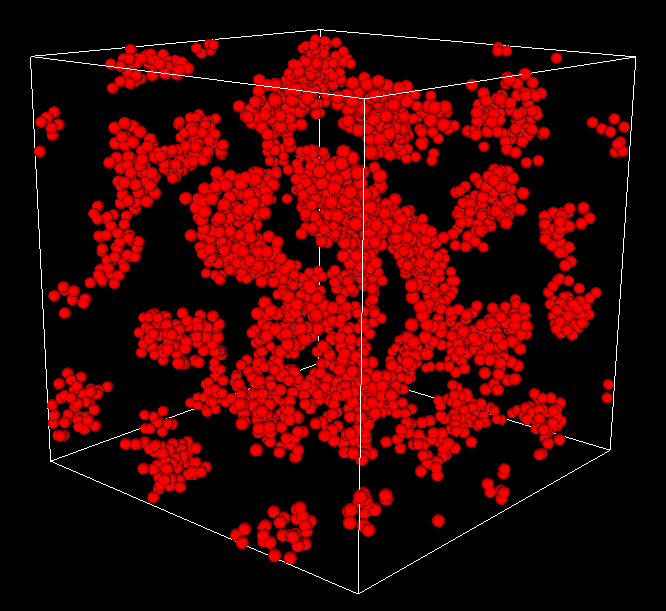
\includegraphics[width=55mm]{./fig/Snap.png}
%	\vspace{-1\baselineskip}
	\label{fig: snap}
	\caption{Snapshot of the Model Network using A1B18A1 Triblock Polymer ($a_{AB} = 80$)}
	\end{center}
\vspace{-2\baselineskip}
\end{wrapfigure}


今回、テレケリックポリマーの計算モデルとして、20 個のビーズから成る A1B18A1 トリブロックポリマーを採用した。
%使用し、トリブロックポリマーの末端が作るクラスターからの引き抜きを観察した。
計算条件は、密度 $\rho =3$ とし、A1B18A1 トリブロックポリマー 1200 本、総ビーズ数は 24,000個とした。


以下の式で表される保存力 $\mathbf{F}_{ij}^C$ に含まれる相互作用パラメータ $a_{ij}$ によって、粒子 $i$ と $j$ 間に働く斥力の大きさが相対位置ベクトル$\mathbf{r}_{ij} (=\mathbf{r}_i - \mathbf{r}_j)$ に依存して決定される。

\begin{equation}
	\mathbf{F}_{ij}^C =
        \begin{cases}
        	a_{ij} w^C (|\mathbf{r}_{ij}|) \dfrac{\mathbf{r}_{ij}}{|\mathbf{r}_{ij}|} & (|\mathbf{r}_{ij}| < r_c) \\
                0 & (|\mathbf{r}_{ij}| \geq r_c)
        \end{cases}
\end{equation}

ここで、$w^C (|\mathbf{r}_{ij}|)$ は粒子間距離に応じて作用を減少させる重み関数であり、 r$_c$ はカットオフ距離を表す。

密度 $\rho =3$ の場合は、非圧縮条件を満たすために、同種ビーズ間の $a_{ii}$ は 25 と設定される。


\begin{wrapfigure}{r}{60mm}
\vspace{-1\baselineskip}
	\begin{center}
	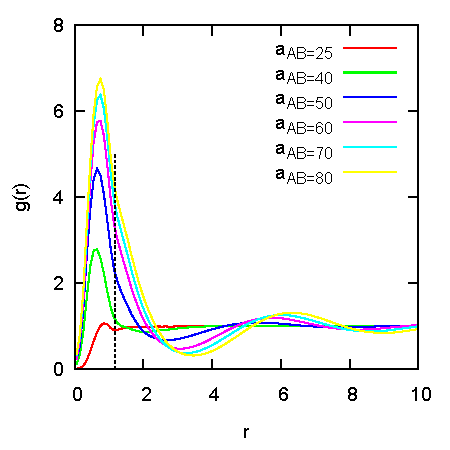
\includegraphics[width=60mm]{./fig/gr_all.pdf}
	\vspace{-1\baselineskip}
	\label{fig: gr}
	\caption{g(r) for A beads with various  $a_{AB}$}
	\end{center}
\vspace{-1.5\baselineskip}
\end{wrapfigure}

以前の検討により、この $a_{ij}$ パラメタは、フローリー・ハギンス格子モデルにおける $\chi$ パラメタと \eqref{eq:achi} 式に示したように相関が取れることが報告されている~\cite{Groot1997}。
\begin{equation}
\dfrac{\chi N k_B T}{\Delta a} = (0.306 \pm 0.003) N
\label{eq:achi}
\end{equation}

この関係を用いて、A, B ビーズ間に斥力を設定($a_{AB} = 25, 40, 50, 60, 70, 80$)し、シミュレーションを行った。
これは、ジブロックポリマーとして考えた場合に、$\chi N \simeq 0 \sim 170$ 程度に対応すると考えることができる。



\section{結果と考察}

Fig.1 に、ポリマー中央部分の B ビーズを透明とし、A ビーズだけを表示したスナップショット ($a_{AB} = 80$) を示した。
なお、十分に初期の緩和計算を行った後であり、末端の A ビーズが偏析したドメインを形成していることが確認できる。

\begin{wrapfigure}{r}{60mm}
\vspace{-3\baselineskip}
	\begin{center}
	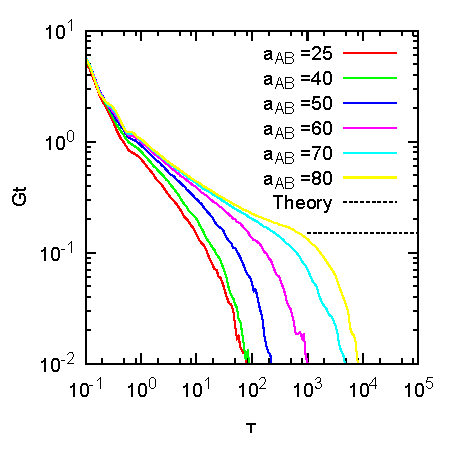
\includegraphics[width=60mm]{./fig/gt_all.pdf}
	\vspace{-1\baselineskip}
	\label{fig: gt}
	\caption{G(t) calculated from autocorrelation of stress with various  $a_{AB}$}
	\end{center}
\vspace{-1.5\baselineskip}
\end{wrapfigure}

種々の $a_{AB}$ における A ビーズの動径分布関数 $g(r)$ を、Fig.2 に示した。
相互作用パラメタの増加に伴い、A ビーズの偏析が進行し、さらに、長距離にわたる構造が形成されることが分かる。

ああああああああああああああああああああああああああああああ
ああああああああああああああああああああああああああああ
ああああああああああああああああああああああああああああああ
ああああああああああああああああああああああああああああ
ああああああああああああああああ

あああああああああああああああああ
ああああああああああああああああああああああああああああああ

長時間領域での終端緩和から、流動に至る緩和時間を見積もることができた。



\begin{wraptable}{r}{60mm}
\vspace{-1.5\baselineskip}
\centering
\caption{$\tau_{e2e}$ and $\tau_{gt}$}
\vspace{5mm}
 \begin{tabular}{|p{3em}|p{3em}|p{3em}|} \hline
\hfil $a_{AB}$ \hfil	&	\hfil $\tau_{e2e}$ \hfil	&	\hfil $\tau_{gt}$ \hfil	\\ \hline \hline
\hfil 25 \hfil 			&	\hfil 48 \hfil				&	\hfil 25 \hfil			\\ \hline
\hfil 40 \hfil			&	\hfil 68 \hfil				&	\hfil 30 \hfil			\\ \hline
\hfil 50 \hfil			&	\hfil 170 \hfil				&	\hfil 63 \hfil			\\ \hline
\hfil 60 \hfil			&	\hfil 650 \hfil				&	\hfil 250 \hfil			\\ \hline
\hfil 70 \hfil			&	\hfil 2200 \hfil			&	\hfil 910 \hfil			\\ \hline
\hfil 80 \hfil			&	\hfil 8200 \hfil			&	\hfil 2500 \hfil		\\ \hline
\end{tabular}
 \label{tbl:t}
\vspace{-1\baselineskip}
\end{wraptable}

\section{おわりに}

DPD 法を用いた粗視化シミュレーションにより、トリブロックポリマーの動的なネットワークの緩和挙動の検討を行い、
偏析度合いの可視化、および、緩和挙動の評価を行った。

相互作用パラメタ $a_{AB}$ の増加に伴い、応力およびポリマー鎖の緩和時間 ($\tau_{gt}, \tau_{e2e}$)は長時間化し、より強固なネットワーク構造の形成が進むことが確認できた。
また、ゴム状平坦部の形成への遷移も確認できた。

ここでは示さなかったが、A ビーズが偏析したドメイン中のビーズの個数の時間変化やブリッジ比についても検討を行っているので、その結果についても併せて議論を行う予定である。

\bibliographystyle{achemso}
%{elsart-num}
%{junsrt-2}
\bibliography{C:/Dropbox/Tex/TeXworks/library.bib}

\end{document}